\documentclass[12pt, letterpaper, oneside, openany]{book}
\usepackage[spanish, english]{babel}
\usepackage{amsthm}
\usepackage[utf8]{inputenc}
\usepackage{csquotes}
\usepackage[margin=25mm]{geometry}
\usepackage[style=apa,doi=false,isbn=false,url=false]{biblatex}
\usepackage{textcomp}
\usepackage{titlesec}
\usepackage{fancyhdr}
\usepackage{color}
\usepackage{graphicx}
\usepackage{setspace}
\usepackage{blindtext}
\usepackage{siunitx}
\usepackage[inline]{enumitem}


\graphicspath{ {Figures/} }
\addbibresource{Thesis.bib}

\onehalfspacing
\setlength{\parskip}{0.5em}

\addto\captionsspanish{
    \renewcommand{\contentsname}
    {Índice}
}

\begin{document}
\begin{titlepage}
    \begin{center}
        
\includegraphics[width=0.18\textwidth]{unam_azul.png}\\
        \textbf{UNIVERSIDAD NACIONAL AUTÓNOMA DE MÉXICO}\\
        MAESTRÍA EN CIENCIAS (NEUROBIOLOGÍA)\\
        INSTITUTO DE NEUROBIOLOGÍA\\
        \vspace{10mm}
        \large
        \textbf{CONECTIVIDAD CEREBRAL EN PACIENTES ADICTOS A COCAÍNA DESPUES DE TRATAMIENTO CON ESTIMULACIÓN MAGNÉTICA TRANSCRANEAL REPETITIVA}\\
        \vspace{10mm}
        \large
        TESIS\\
        \normalsize
        QUE PARA OPTAR POR EL GRADO DE:\\
        MAESTRA EN CIENCIAS\\
        \vspace{10mm}
        PRESENTA:\\
        \large
        \textbf{SOFÍA FERNÁNDEZ LOZANO}\\
        \vfill
        \normalsize
        TUTOR PRINCIPAL\\
        EDUARDO ADRIÁN GARZA VILLARREAL\\
        INB, UNAM\\
        \vspace{3mm}
        MIEMBROS DEL COMITÉ TUTOR\\
        SARAEL ALCÁUTER SOLÓRZANO\\
        INB, UNAM\\
        \vspace{1mm}
        ISRAEL VACA PALOMARES\\
        FP, UNAM\\
        \vspace{5mm}
        QUERÉTARO, MÉXICO, 2019
    \end{center}
\end{titlepage}


\pagestyle{empty}
\begin{center}
    \large
    Universidad Nacional Autónoma de México\\
    Instituto de Neurobiología\\
\end{center}

\vspace{1cm}
\normalsize
Los miembros del Jurado certificamos que la tesis elaborada por:
\textbf{Sofía Fernández Lozano}, cuyo título es:
\textbf{``Conectividad Cerebral en Pacientes Adictos a Cocaína después
de Tratamiento con Estimulación Magnética Transcraneal Repetitiva''} se
presenta como uno de los requisitos para obtener el grado de Maestría en
Ciencias (Neurobiología) y cumple con los criterios de originalidad y calidad
requeridos por la División de Estudios de Posgrado de la Universidad Nacional
Autónoma de México.

\vfill

\begin{flushright}
    \large
    Firma
\end{flushright}

\begin{flushleft}
    Presidente\\
    Dr.\hrulefill\\
    \vspace{3mm}
    Secretario (Tutor)\\
    Dr.\hrulefill\\
    \vspace{3mm}
    Vocal\\
    Dr.\hrulefill\\
    \vspace{3mm}
    Suplente\\
    Dr.\hrulefill\\
    \vspace{3mm}
    Suplente\\
    Dr.\hrulefill\\
\end{flushleft}

\vspace{1cm}

\begin{center}
    Aprobado por el Comité Académico\\
    \vspace{15mm}
    \makebox[7cm]{\hrulefill}\\
    Coordinador del Programa
\end{center}
\newpage

\begin{flushright}
    \null\vspace{\stretch{1}}
    \emph{A todas las poblaciones marginalizadas\\que estamos tomando nuestra voz en las ciencias.}
    \vspace{\stretch{2}}\null
\end{flushright}
\newpage

\begin{center}
    \huge\textbf{Agradecimientos}
\end{center}

A la \emph{Universidad Nacional Autónoma de México (UNAM)} y al \emph{Instituto de Neurobiología (INB)}, así como a la \emph{Facultad de Psicología} y su \emph{Unidad de videoconferencias}, por permitirme desarrollarme bajo sus enseñanzas.

Al \emph{Consejo Nacional de Ciencia y Tecnología (CONACYT)} (Becario {\textnumero} 858808 y Proyecto FOSISS {\textnumero} 0260971) por su apoyo económico y patrocinio al proyecto de investigación del que formé parte.

Al \emph{Instituto Nacional de Psiquiatría "Ramón de la Fuente Muñiz"}, su \emph{Clínica de Adicciones} y \emph{Unidad de Imagenes Cerebrales}, así como su equipo de psiquiatras, enfermeras y participantes, sin quienes este trabajo no hubiera sido posible.

A \emph{Eduardo Garza}, por desde un principio enseñarme a aprender por mí misma; darme las herramientas para llegar hasta donde estoy y su invaluable guía todo este camino.

A \emph{Sarael Alcauter} e \emph{Israel Vaca}, por sus comentarios y observaciones, sus enseñanzas y, sobretodo, por creer en este trabajo.

A \emph{Said}, \emph{Diego}, \emph{Viviana}, \emph{Alan}, y el resto del \emph{GarzaLab}, por todas las tardes (y noches) que me acompañaron dentro y fuera de la oficina; por enseñarme que la ciencia puede ser divertida.

A \emph{mis compañeros de Psicología y FESI}, por las pláticas, el apoyo mutuo; ser un equipo.

A \emph{Dardo, Nora y Ehsan}, por sus invaluables enseñanzas y comentarios; a \emph{Ariel, Rui, Luana, Joseph, Wenjing, Gene-Jack, Peter, Corinde, y todo el equipo del LNI}, por hacerme sentir bienvenida y compartir conmigo 2 meses maravillosos llenos de aprendizaje.

A \emph{mis padres y mis hermanos} que desde Tijuana me mandaron todo su apoyo y cariño, y sin quienes nunca hubiera llegado hasta donde estoy.

A \emph{Eusebio, Paola A, Jessica, Paola S y Catherine} por seguir estando desde la carrera.

A \emph{Monica} por su valiosa amistad, a pesar del tiempo y la distancia; por creer en mí.

A \emph{Yaaj México}, por darme una segunda familia.

A \emph{Fausto}, por su compañia y guía, por recordarme enfocarme en mí antes que nadie más.

A \emph{Sonny}, por llegar en el momento justo y recordarme cómo sonreír cuando más lo necesitaba.\newpage



\frontmatter
\pagestyle{plain}
\chapter*{\center Resumen}
\addcontentsline{toc}{chapter}{Resumen Español}
\selectlanguage{spanish}
\begin{center}
    \large\textbf{Conectividad Cerebral en Pacientes Adictos a Cocaína después de
     Tratamiento con Estimulación Magnética Transcraneal Repetitiva}
\end{center}
\begin{quotation}
    \noindent
Aún hay poca e inadecuada investigación sobre la efectividad de la estimulación magnética transcraneal repetitiva (EMTr) como tratamiento para la dependencia a cocaína. En este estudio clínico longitudinal, mono-céntrico, doble-ciego exploramos las diferencias en topología entre pacientes con adicción a cocaína y controles sanos y usamos estos datos para evaluar los cambios clínicos y de topología después de un tratamiento de EMTr sobre la corteza prefrontal dorsolateral. La topología global y escalas clínicas fueron medidas en 40 participantes antes y después de recibir dos sesiones diarias de EMTr real o sham por dos semanas; así como después de recibir sesiones semanales de mantenimiento por tres ($n=16$) y seis meses ($n=11$). Nuestro análisis preliminar mostró diferencias significativas en el costo, eficiencia y cualidad de pequeño-mundo entre las redes de nuestros pacientes y sujetos controles. Modelos de efectos mixtos mostraron una interacción significativa entre el grupo de estimulación y la fase de tratamiento tanto para el craving como impulsividad. Hubo también cambios significativos en el costo y la métrica de pequeño mundo de las redes atribuibles al tratamiento de EMTr. Todos estos cambios se mantuvieron después de los tres meses de mantenimiento y no fue hasta los seis meses de mantenimiento que empezaron a mostrar un decaimiento. Estos resultados proveen evidencia de la eficacia de la EMTr como una alternativa de tratamiento en la adicción así como la posibilidad de utilizar metodología de teoría de grados para la exploración de la naturaleza, evolución y tratamiento de la adicción.
\end{quotation}
\clearpage


\chapter*{\center Abstract}
\addcontentsline{toc}{chapter}{Resumen Inglés}
\selectlanguage{english}
\begin{center}
    \large\textbf{Brain Connectivity in Cocaine-addicted Patients after Repetitive Transcranial Magnetic Stimulation Treatment}
\end{center}
\begin{quotation}
    \noindent
    There is still few and inadequate research being done on the effectivity of repetitive transcranial magnetic stimulation (rTMS) as a treatment for cocaine addiction and even fewer using graph theory analysis methods in the study of addiction. In this longitudinal, monocentric, double-blind placebo controlled clinical trial, we explored the topology differences between cocaine-dependent participants and healthy controls and used that data to assesss the clinical and topological changes after a rTMS treatment over the left dorsolateral prefrontal cortex. The global topology and clinical metrics were measured in 40 cocaine-dependent, treatment seeking participants before and after receiving two daily sessions of either real or sham rTMS for two weeks. We also explored these same measures after receiving weekly maintenance sessions for three ($n=16$) and  six months ($n=11$). Our preliminary analysis showed significant difference in the cost, efficiency and small-worldness of the networks between our sample of cocaine-dependent participants and healthy controls. Mixed effects models showed a significant interaction of stimulation group and stage of treatment for both craving and impulsivity. There were significant changes in the cost of the networks and the small-worldness attributable to the rTMS treatment. All of these changes were mantained after the three months of maintenance sessions and showed slight decay by the sixth month. These results provide evidence for the efficacy of rTMS as a promising alternative treatment for addiction as well as the appropriateness of graph theory analyses methods for the exploration of the nature, evolution and treatment of addiction.
\end{quotation}
\clearpage
\selectlanguage{spanish}

\tableofcontents

\mainmatter
\definecolor{gray42}{gray}{0.42}
\newcommand{\hsp}{\hspace{15pt}}
\titleformat{\chapter}[hang]{\Huge\bfseries}{\thechapter\hsp\textcolor{gray42}{\textbar}\hsp}{0pt}{\Huge\bfseries}

\chapter{Introducción}
El abuso de drogas ilícitas es uno de los problemas de salud pública más
importantes del país y del mundo.
El consumo de sustancias produce alteraciones plásticas en el
cerebro que pueden desencadenar consecuencias graves para la salud y funcionalidad
social de los consumidores. \par
A pesar de esto, el tratamiento existente para la dependencia a las sustancias es insuficiente e ineficiente.
Con un enfoque centrado en listas de síntomas y patrones de consumo, contados tratamientos farmacológicos aprobados por la FDA\footnote{Ninguno para la dependencia a cocaína.}
y una tasa de recaída cercana al 50\%, la búsqueda de nuevos y mejores enfoques de tratamiento es imperativa.\par
Es necesario aprovechar el avance en el entendimiento de los mecanismos neurobiológicos del cerebro adicto para el establecimiento de biomarcadores de la adicción y desarrollo de estrategias más eficientes de tratamiento.\par
Uno de estos nuevos enfoques es la estimulación magnética transcraneal repetitiva (EMTr). Se ha visto que esta, por medio de pulsos electromagnéticos que estimulan el funcionamiento de la corteza prefrontal, permite un mejor manejo del \textit{craving}\footnote{Sensación de deseo intenso hacia el consumo de la sustancia.}, la impulsividad y la sintomatología afectiva de la adicción. \par
No obstante, son limitados aún los estudios que comprueban su eficacia clínica como tratamiento; son realizados con base en diseños exploratorios, carecen de un grupo control o exploración neurobiológica o sus muestras son muy pequeñas.\par
Proponemos entonces con el presente proyecto, un estudio de diseño mixto donde se amplien los conocimientos actuales sobre las bases neurobiológicas de la adicción al mismo tiempo que se compruebe la eficacia de la estimulación magnética transcraneal repetitiva como un tratamiento para la dependencia a la cocaína.\par
Primero, en un diseño transversal comparamos las redes de conectividad funcional de pacientes dependientes a cocaína con las de un grupo pareado de controles sanos con el fin de ampliar los conocimientos actuales sobre la organización topológica del cerebro adicto.\par
En este análisis observamos diferencias en la topología global del cerebro adicto, en donde este se encuentra hiperconectado pero con menores índices de cualidad de pequeño mundo que aquellas redes de los sujetos controles sanos.\par
Bajo un diseño longitudinal monocéntrico a doble ciego, evaluamos los efectos clínicos del tratamiento de estimulación magnética transcreneal repetitiva a \SI{5}{\hertz} sobre la corteza prefrontal dorsolateral. En este análisis encontramos un efecto significativo de mejoría clínica a dos semanas tanto de la sensación subjetiva de \textit{craving} expresada por medio de una escala visual análoga como de la medida de impulsividad explorada por la escala de impulsividad de Barratt. Notamos diferentes patrones de mejoría relativos al estado basal de los participantes y, aunque esta mejoría clínica se mantuvo a los 3 meses de mantenimiento, en la medición posterior a los seis meses de mantenimiento comenzamos a notar una atenuación e incluso empeoramiento de los efectos clínicos principalmente en aquellos sujetos que comenzaron con una sintomatología disminuida. \par
De igual forma, utilizando las mismas técnicas de neuroimagen funcional y teoría de grafos, exploramos la topología de redes funcionales en las diferentes etapas del estudio para observar los efectos del tratamiento sobre los neurocircuitos cerebrales y asociar la mejoría clínica con los cambios en la neurobiología cerebral. Aunque la asociación con las escalas clínicas no fue tan directa como esperaríamos, notamos un efecto paralélo a la mejoría clínica donde la hiperconectividad disminuía a causa del tratamiento de estimulación magnética del mismo modo que la cualidad de pequeño mundo aumentaba. Estos efectos se mantuvieron en las mediciones posteriores a las sesiones de mantenimiento. \par
Nuestros resultados aportan evidencia sobre la efectividad del tratamiento de estimulación magnética transcraneal en la sensación de \textit{craving} e impulsividad en pacientes adíctos, así como demostrar que los análisis globales cerebrales y aquellos basados en técnicas de teoría de grafos pueden ser adecuados para la exploración de la naturaleza, evolución y tratamiento de la adicción.



\chapter{Antecedentes}
\section{Adicción a Cocaína}
% Buscar mas sobre bases biológicas de Adicción
% Agregar impulsividad
La adicción es una consecuencia patológica del aprendizaje sobre recompensas, donde se alteran las rutas meso-córtico-límbicas de la dopamina \parencite{Volkow2016}.
El término de adicción es usado para indicar la etapa más severa y crónica del trastorno por consumo de sustancias, donde hay una pérdida substancial de auto-control \parencite{Volkow2016}.
En México se ha reportado un aumento en la prevalencia del 1.8\% con respecto al consumo de cualquier droga para la población de 12 a 65 años, agregándose 100,000 personas como dependientes (de 450,000 el 2008 a 550,000 en el 2011)\parencite{InstitutoNacionaldePsiquiatriaRamondelaFuenteMuniz2012a}.
La adicción es entonces un trastorno recurrente que puede caracterizarse por:
\begin{enumerate*}
    \item{compulsión en buscar y consumir la sustancia; }
    \item{pérdida de control limitando el consumo, y; }
    \item{emergencia de un estado emocional negativo reflejando un síndrome motivacional de abstinencia}
\end{enumerate*}.
Por lo que puede dividirse en tres estados: intoxicación, abstinencia y afecto negativo, y, \textit{craving} \parencite{Koob2010a}.\par
El \textit{craving}, o el deseo fuerte e intenso de consumir la sustancia, tanto para volver a sentir los efectos eufóricos como para evitar los aspectos de abstinencia provocados por su ausencia, es un elemento clave en la recaída \parencite{Koob2010a}.
Existe una baja regulación de señalización de dopamina (DA) en regiones prefrontales del cerebro y sus circuitos asociados, afectando los procesos ejecutivos \parencite{Goldstein2012a}.
Esto crea un desbalance que es crucial tanto para el desarrollo gradual del comportamiento compulsivo como para la asociada inhabilidad a resistirse a las fuertes ansias por consumir o para seguir las decisiones de parar tomando la droga \parencite{Volkow2016}.
El \textit{craving} es entonces, por estas características, un punto clave como enfoque para el tratamiento de las adicciones.

\section{Tratamiento para la Adicción a la Cocaína}
Actualmente no existe una cura para la adicción.
El tratamiento consiste en un abordaje multidisciplinario que ayuda al manejo de la enfermedad.
Generalmente este consiste en el apoyo psicoterapéutico, consejería y tratamiento farmacológico en conjunto. \par
No obstante, la naturaleza crónica de la adicción hace que la recaída no sea solo posible, sino probable \parencite{NIDA.}.
Estudios de seguimiento a 1 año postratamiento han encontrado que solo del 40-60\% se mantienen en abstinencia \parencite{McLellan1980} \footnote{Datos de tratamientos en EEUU}.\par
Debido a esto es de suma importancia la revisión del manejo actual de la adicción y la búsqueda de nuevos tratamientos alternativos que sean más efectivos.

\subsection{Tratamiento farmacológico}
No existe actualmente un tratamiento farmacológico aprobado por la FDA (Administración de comida y drogas, por sus siglas en inglés) de Estados Unidos para la dependencia a la cocaína.
Los medicamentos utilizados comúnmente son los mismos que aquellos usados para tratar la epilepsia o los espasmos musculares, principalmente con el fin de aliviar la ansiedad y la agitación resultantes de la adicción a la cocaína.
Algunos de estos son: gabapentina, un anticonvulsivante análogo a GABA; modafinilo, promueve el estado de alerta inhibiendo la recaptura de dopamina; topiramato, anticonvulsivante que alivia la agitación; vigabatrina, anti-epiléptico usado para el \textit{craving}inhibiendo el catabolismo de GABA; y, baclofeno, relajante muscular agonista de GABA \parencite{Volkow2007b}.\par
De todos los medicamentos usados para tratar la adicción a la cocaína, disulfiram es el que ha tenido más resultados exitosos consistentes \parencite{Volkow2007b}.
Usualmente utilizado como tratamiento a la adicción al alcohol por medio de la inducción de una reacción adversa al alcohol, disulfiram también a sido prescrito para desalentar el uso de la cocaína.
Aún no se conoce específicamente como funciona, pero sus efectos pueden estar relacionados a su capacidad de inhibir una enzima que convierte a la dopamina en noradrenalina.
Sin embargo, no es efectivo para todas las personas, ya que se ha visto que ciertas variaciones genéticas influyen en la efectividad del tratamiento \parencite{Gaval-Cruz2009a, Volkow2007b}.\par

\subsection{Tratamiento comportamental}
Junto al tratamiento farmacológico, usualmente se lleva a cabo un abordaje comportamental por medio de psicoterapia y consejería.
Entre los modelos más utilizados dentro de estas áreas están:
la psicoterapia cognitivo-conductual, donde el paciente aprende a identificar y corregir comportamientos problemáticos aplicando una serie de técnicas que pueden ser usadas para detener el abuso de la sustancia y abordar los problemas que suelen ocurrir en conjunto;
el manejo de contingencias, donde por medio de recompensas tangibles se refuerzan los comportamientos positivos como la abstinencia;
intervención motivacional, es un abordaje de consejería donde se ayuda al paciente a resolver su ambivalencia sobre el compromiso al tratamiento y parar el consumo de la sustancia;
y la terapia familiar conductual, que intenta abordar no solo el consumo de la droga, sino también los problemas en conjunto, como trastornos de conducta, maltrato infantil, depresión, conflictos familiares y desempleo \parencite{Volkow2008}.

\section{Estimulación Magnética Transcraneal Repetitiva}
% Buscar estudios de Hanlon
% Agregar subsección de TMS como tratamiento de adicción???
A pesar de ser originalmente desarrollada como una herramienta diagnóstica, la Estimulación Magnética Transcraneal (EMT) puede modular, transitoria ---o duraderamente--- la excitabilidad cortical por medio de la aplicación de pulsos electromagnéticos localizados\parencite{Horvath2011a}.\par
La EMT repetitiva (EMTr) es una variación de la EMT donde la estimulación es provista en varias sesiones con las mismas condiciones para crear excitación o inhibición a largo plazo en la corteza cerebral.
En EMTr las actividades eléctricas en el cerebro son influenciadas por los campos magnéticos. La inducción electromagnética generada por EMTr es indolora y pasa sin daño por la piel y el cráneo \parencite{Noohi2016}.
Se ha demostrado que la EMTr puede perturbar la actividad neuronal por períodos que exceden la duración de la estimulación; por lo tanto, es una técnica de neuromodulación que produce cambios plásticos \parencite{Horvath2011a}.\par
EMTr sobre la Corteza Prefrontal (CPF) ha mostrado tener efectos moduladores en los sistemas dopaminérgicos mesolímbicos y mesoestriatales.
Se encontró que la Emtr de alta frecuencia sobre la CPF inducía liberación subcortical de dopamina (DA) en el núcleo caudado\parencite{Strafella2001}.
La EMTr sobre la Corteza Prefrontal Dorsolateral (DLPFC) izquierda modula la liberación de DA en: Corteza Anterior Cingulada (CAC) y Corteza Orbitofrontal (COF) en el mismo hemisferio que la estimulación \parencite{Cho2009}.
Sesiones repetidas de EMTr sobre la CPF son sugeridas para reducir el \textit{craving}, búsqueda de drogas y, eventualmente, el consumo y recaída\parencite{Amiaz2009}.\par
\textcite{Bellamoli2014a} realizaron una revisión de la literatura buscando protocolos de EMTr sobre el \textit{craving} y consumo de nicotina, alcohol y cocaína. Basándose en la evidencia encontrada, concluyeron que la EMTr puede ser clasificada como probablemente efectiva en el tratamiento de la adicción.
Las características neuromoduladoras y los cambios plásticos observados como efecto de la EMTr hacen de esta un tratamiento efectivo factible para alterar los circuitos involucrados en el \textit{craving} de la adicción, lo que, por efecto, llevaría a la disminución de la recaída y una mayor efectividad de tratamiento.

\section{Conectividad Funcional en la Adicción}
% Separar Bases de FMRI y FMRI en adicción como subsección
% Agregar bases de resonancia magnética
Mucho de lo que actualmente se conoce sobre función cerebral ha venido de estudios donde se miden los cambios en actividad neuronal y conducta después de la administración de una tarea o estímulo (\textit{task-based fMRI}), sin embargo, cambios espontáneos de la señal BOLD que no son atribuidos a un diseño experimental también están presentes \parencite{Fox2007}.
Es así como la resonancia magnética funcional en estado de reposo (\textit{resting-state fMRI} o RS-RMf) ha emergido recientemente como una poderosa herramienta que permite medir la conectividad funcional \parencite{Biswal2010}\par
La resonancia funcional durante el reposo revela fluctuaciones espontáneas de gran amplitud y baja frecuencia ($<0.1 Hz$) que pueden ser temporalmente correlacionadas entre áreas relacionadas funcionalmente.
Un único escaneo (de al menos 5 minutos) puede ser usado para estudiar una multitud de circuitos funcionales simultáneamente \parencite{Biswal2010}.\par
% Aquí empieza neuroimagen y adicciones
Las investigaciones de neuroimagen sobre la neurobiología de las adicciones han sido en su mayoría realizadas por técnicas como la tomografía por emisión de positrones (PET) o la RMf por medio de tareas, donde muchas de estas tareas tienen que ver con la presentación de señales o impulsos relacionados con la sustancia \parencite{Jasinska2014}. Actualmente son pocos los estudios de conectividad funcional en estado de reposo en el campo de las adicciones, especialmente comparados con los que utilizan las técnicas anteriores. \par
Relacionado al abuso de la heroína, se ha encontrado alteraciones en la conectividad funcional entre regiones límbicas ---como el Núcleo Accumbens (NA), amígdala, Núcleo Caudado (NC)--- y regiones frontales ---como la COF y el cíngulo\parencite{Ma2010,Tianye2015,Wang2010,Zhang2016}.\par
Son especialmente pocas las investigaciones que han reportado la conectividad funcional de reposo en la adicción a la cocaína.
En estos pacientes se ha observado una disminución en la conectividad del sistema meso-cortico-límbico (MCL); entre el Área Tegmental Ventral (ATV) y el NA, y el Tálamo; entre la Amígdala y la CPF medial; así como entre el Hipotálamo y la CPF medio-dorsal.
Esta disminución en conectividad estaba negativamente relacionada con el tiempo de adicción \parencite{Gu2010}.
De igual forma, se ha encontrado una correlación negativa entre el \textit{craving} subjetivo y la actividad del giro medial-posterior del cíngulo en adictos a la cocaína.
En el mismo estudio se observó una relación entre las áreas que procesan las señales relacionadas a la droga (COF y estriado ventral);
así como una conectividad negativa entre estas áreas y el giro medial posterior del cíngulo \parencite{Wilcox2011}.\par
Se han reportado diferencias interhemisféricas en las regiones frontales entre consumidores y sujetos control; así como una reducción en la conectividad funcional interhemisférica entre nodos de la red de atención dorsal (áreas latero-frontales bilaterales, premotoras mediales y parietales posteriores), lo que podría sugerir que estas anormalidades se relacionan a los problemas de atención presentados comúnmente en la adicción \parencite{Kelly2011a}.
\textcite{Verdejo-Garcia2014} hallaron menor conectividad funcional entre CAC, tálamo, ínsula y tallo cerebral; así como alteraciones funcionales en los sistemas fronto-límbicos.\par
\textcite{Hu2015} encontraron una conectividad aumentada en los circuitos fronto-estriatales de los usuarios de cocaína, los cuales también presentaron una conexión reducida entre el estriado y las regiones del cíngulo, estriado, hipocampo/amígdala e ínsula. El uso compulsivo de la cocaína fue asociado con un balance entre un aumento de la conectividad anteroestriatal-prefrontal/orbital y una disminución de la conectividad estrato-dorsal anterior cingulada.\par
Los primeros estudios de conectividad efectiva en usuarios de cocaína en abstinencia encontraron una mayor conectividad del ATV a: NA, hipocampo y CFM; así como una menor conectividad de la CFM a ATV y del NA a CFM.
A las 72 horas de abstinencia, los fumadores de cocaína presentaron conexiones causales (dirigidas) hacia regiones límbicas, mediales y frontales del sistema MCL que no se presentaron en los controles \parencite{Ray2017,Ray2016}.\par
Estos estudios de neuroimagen y conectividad permiten tener una visión de los circuitos involucrados en la adicción, así como un marco de referencia para evaluar el cambio producido por el tratamiento.
% Resumir los circuitos mencionados? Podría ser intro para las redes seleccionadas
\subsection{Teoría de Grafos}
La teoría de grafos es un nuevo enfoque que ha venido tomando fuerza en el campo de la neuroimagen como una forma de describir comprensivamente la red de elementos y conexiones que forman el cerebro humano.
Un grafo es una representación de una red. Consiste en un conjunto de vértices o nodos y un conjunto de \textit{edges} o aristas. La presencia de una arista entre dos vértices indica la presencia de algún tipo de interacción o conexión \parencite{Stam2007}.
Tanto redes estructurales como funcionales pueden ser exploradas usando teoría de grafos; las métricas de la red pueden ser computadas para extraer las características de la topología del grafo.
Esta topología se presta para ser comparada entre sujetos o grupos de investigación \parencite{Bullmore2009a,Sporns2011}.\par
Se ha apreciado que muchos trastornos neurológicos y psiquiátricos pueden ser descritos como síndromes de disconectividad.
Una aplicación de la teoría de grafos en este contexto puede ser el de proveer nuevas medidas para cuantificar diferencias entre grupos de pacientes y grupos apropiados de comparación \parencite{Bullmore2009a}.

\subsubsection{Medidas topográficas}
Buscar formulas de métricas y su referencia
La topología de una red o grafo puede describirse por medio de diversas métricas. Las principales medidas para describir las redes cerebrales pueden clasificarse en las siguientes categorías.\par
\theoremstyle{definition}
\newtheorem*{def1}{Costo}
\newtheorem*{def2}{Segregación}
\newtheorem*{def3}{Integración}
\newtheorem*{def4}{Pequeño Mundo}
El número de conexiones de cada nodo(grado de conectividad). El grado medio de todos los nodos refleja la densidad de la red.


\chapter{Planteamiento del problema}
\section{Justificación}
La adicción a sustancias es un importante problema de salud pública en México y en el mundo.
En México se ha reportado un aumento significativo en el consumo de drogas ilícitas en los últimos años, aumentando del 7.2\% en el 2011 al 9.9\% de la población total en el 2016.
La dependencia a drogas\footnote{Reportada en el último año.} fue reportada por un 0.6\% de la población \textemdash{}1.1\% de hombres y 0.2\% de mujeres en el 2016.
De estas drogas ilícitas, la cocaína ocupa el segundo mayor lugar en su consumo, después de la mariguana \parencite{Villatoro-Velazques2017}.\par
Aunque la mariguana sea la droga de mayor consumo, el presente proyecto se enfoca en la dependencia a la cocaína debido a su mayor efecto adictivo\footnote{Esto se observa en un mayor y más intenso \textit{craving}.} e impacto sobre la salud y funcionalidad social de sus usuarios, tanto a corto como largo plazo. \par
El tratamiento actual para la adicción, específicamente para la dependencia a cocaína, es insuficiente.
El campo de la psiquiatría principalmente se apoya de listas de síntomas y marcadores de consumo.
Hasta el momento no hay biomarcadores clínicos útiles para la adicción a sustancias.
Un pobre entendimiento del cerebro humano adicto y de los efectos complejos de las drogas en los distintos mecanismos neurobiológicos y circuitos neuronales son las razones principales de la falla de desarrollar tratamientos efectivos, ya que el tratamiento habitual presenta una tasa de recaída cercana al 50\% \parencite{McLellan2000a}. \par
Una nueva propuesta de tratamiento que pretende aprovechar las investigaciones recientes en los neurocircuitos de la adicción es el de la EMTr.
Con base en la involucración de la mediación frontal sobre la respuesta al craving, esta zona puede funcionar como un objetivo terapéutico. Intervenciones como la EMTr que refuerzan a un debilitado pero aún funcional circuito fronto-accumbal pueden incrementar la habilidad de usuarios a cocaína para bloquear o reducir la respuesta al \textit{craving} \parencite{Volkow2010a}. \par
Varios investigadores han buscado explorar la eficacia de este tratamiento con resultados prometedores en la reducción clínica del craving \parencite{Rachid2018}.
No obstante, los estudios son aún insuficientes; muy pocos de los estudios clínicos cuentan con un grupo control de comparación y estos son diseños ciegos sencillos \parencite{Kearney-Ramos2018a, Kearney-Ramos2019, Terraneo2016,Hanlon2015}.
El único estudio doble-ciego contaba con una muestra de solo 10 sujetos \parencite{Bolloni2016}.
Y, aunque se ha demostrado que las medidas de neuroimagen son más sensibles para detectar diferencias de grupo en valencia o agitación ante estímulos \parencite{Goldstein2012a} y capaces de predecir la recaída y respuesta a tratamiento \parencite{Suckling2017}, solamente tres de los estudios clínicos de EMTr exploraban medidas cerebrales con neuroimagen \parencite{Kearney-Ramos2018a, Kearney-Ramos2019, Hanlon2015}. \par
\textcite{Steele2018} argumentan que para diagnosticar y tratar efectivamente a los pacientes adictos a sustancias, en vez de enfocarse en una región cerebral o neurotransmisor específico, como se ha venido realizando los últimos años, un mejor entendimiento de los efectos de la condición sobre la organización topológica y las redes de conectividad cerebral puede tener una mucho mayor importancia estratégica. \par
Es por eso que en el presente proyecto, se pretende evaluar la efectividad del tratamiento con EMTr en adicción a la cocaína, siguiendo los lineamientos de \textcite{Ekhtiari2019}, en un estudio doble-ciego a largo plazo (dos semanas de tratamiento agudo; tres y seis meses de mantenimiento) y explorar los efectos en mejoría clínica y sobre la topología de las redes de conectividad cerebral.

\section{Pregunta de investigación}
¿Existen cambios en la topología de redes de conectividad funcional en pacientes con adicción a la cocaína después de un tratamiento de estimulación magnética transcraneal repetitiva a corto y largo plazo?

\section{Objetivos}
\subsection{General}
\begin{enumerate}[label=General., left= \parindent]
    \item Evaluar los cambios en conectividad cerebral funcional utilizando métodos de teoría de grafos y su posible relación con la mejoría clínica después de un tratamiento con estimulación magnética transcraneal repetitiva en pacientes con adicción a cocaína (dos semanas) y sesiones de mantenimiento a largo plazo (tres y seis meses) y su relación con la topología de redes en pacientes sanos.
\end{enumerate}
\subsection{Específicos}
\begin{enumerate}[label=Específico \arabic*., left= \parindent]

    \item Comparar la topología de redes entre los pacientes diagnosticados con adicción a la cocaína y un grupo de controles sanos.
    \item Ver si existe una mejoría clínica después de dos sesiones de tratamiento de EMTr
    \item Comprobar si la mejoría se mantiene con sesiones de mantenimiento semanales de EMTr (tres y seis meses).
    \item Observar si existen cambios en la topología de redes después del tratamiento y sesiones de mantenimiento de EMTr.
    \item Buscar si existe una relación entre los cambios sintomáticos y de topología después del tratamiento y mantenimiento de EMTr.
\end{enumerate}

\section{Hipótesis}
\subsection{Clínicas}
\begin{enumerate}[label=Hipótesis \arabic*., left= \parindent]
    \item Habrá una disminución en el \textit{craving} atribuible al tratamiento de EMTr a las dos semanas, tres y seis meses en comparación con la medición basal.
    \item Habrá una disminución en la medida de impulsividad atribuible al tratamiento de EMTr a las dos semanas, tres y seis meses en comparación con la medición basal.
\end{enumerate}
\subsection{Topológicas}
    \subsubsection{Basales}
    \begin{enumerate}[resume,label=Hipótesis \arabic*., left= \parindent]
        \item Los pacientes con adicción presentarán mayor hiperconectividad (\emph{fuerza} y \emph{densidad}) en sus redes de conectividad que los controles sanos.
        \item Las redes de conectividad en pacientes adictos presentarán menores índices de eficiencia (\emph{escalar de pequeño-mundo} y \emph{eficiencia local} y \emph{global}) que las de los controles sanos.
    \end{enumerate}
    \subsubsection{Relacionadas con EMTr}
    \begin{enumerate}[resume,label=Hipótesis \arabic*., left= \parindent]
        \item La conectividad de la red (\emph{fuerza} y \emph{densidad}) disminuirá con el tratamiento real de EMTr en comparación con \textit{sham}.
        \item La eficiencia de la red (\emph{eficiencia local}, \emph{global} y \emph{pequeño-mundo}) aumentará con el tratamiento real de EMTr en comparación del \textit{sham}.
    \end{enumerate}
    \subsubsection{Relacionadas con mejoría clínica}
    \begin{enumerate}[resume,label=Hipótesis \arabic*., left= \parindent]
        \item La disminución en conectividad de red estará asociada a una disminución en \textit{craving}.
        \item El aumento en eficiencia de la red estará asociado a una disminución en \textit{craving}.
        \item La disminución en conectividad de red estará asociada a una disminución en impulsividad.
        \item El aumento en eficiencia de la red estará asociado a una disminución en impulsividad.
    \end{enumerate}



% \chapter{Sujetos, material y métodos}
% Este fue un estudio monocéntrico doble-ciego controlado por placebo y de grupos paralelos y fue llevado a cabo en su totalidad en la Subdirección de Investigaciones Clínicas del Instituto Nacional de Psiquiatría Ramón de la Fuente Muñiz (INPRFM) en la Ciudad de México.\par
La investigación forma parte de un proyecto mayor financiado por CONACYT:
``Cambios en la estructura y conectividad funcional cerebrales relacionados a la mejoría clínica en pacientes con adicción a la cocaína después de un tratamiento con estimulación magnética transcraneal'',
clave S0008-2015-2-260971, bajo la dirección del doctor Eduardo Garza Villarreal y aprobado por el Comité de Ética del INPRFM (CEI/C/070/2016).

\section{Muestra}
Para el presente proyecto, tanto pacientes de la clínica de adicciones del INPRFM como externos que cumplieran con el diagnóstico de dependencia de cocaína (F14.2x) del DSM 5 \parencite{APA2013} fueron reclutados para participar en el ensayo clínico.\par
Cuarenta y seis sujetos fueron asignados aleatoriamente a los distintos grupos de estimulación (Figura \ref{fig:flow}).
Un grupo recibió estimulación sobre la corteza prefrontal dorsolateral izquierda y el otro, un protocolo sham de estimulación simulada sobre la misma área.

\subsection{Grupo control}
Para la realización del análisis transversal de pacientes adictos y controles sanos, los datos de neuroimagen de una submuestra de 45 sujetos sanos fueron retomados de la base de datos de un proyecto realizado con anterioridad en el INPRFM \parencite{Garza2017}.
Debido a que la cantidad total de los sujetos sanos de la base de datos de ese estudio es menor al número de participantes reclutados para nuestro proyecto fue imposible parear ambos grupos.

\begin{figure}[H]
    \centering
    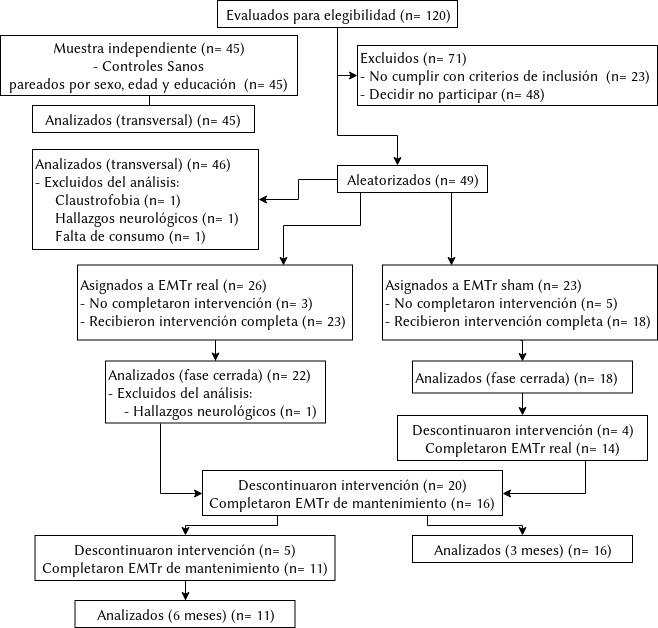
\includegraphics[width=\textwidth]{participantFlow}
    \caption{Diagrama de flujo de participantes}
    \label{fig:flow}
\end{figure}

\section{Criterios de selección}
Se siguieron los criterios de selección establecidos en el proyecto principal.
Estos fueron propuestos con la intención de disminuir la posibilidad de aparición de cualquier variable extraña y de seguir los lineamientos de seguridad tanto para la MRI como la EMTr.

\subsection{Criterios de inclusión}
Todos los participantes debían cumplir con los siguientes criterios para ser registrados en el estudio y ser asignados a uno de los grupos de investigación
\begin{enumerate*}[label=\emph{\alph*}), before=\unskip{: }, itemjoin={{; }}, itemjoin*={{, y }}]
    \item tener una edad mínima de 18 años y máxima de 50 años
    \item ser usuario de cocaína durante al menos dos  años, con un uso promedio actual mínimo de tres veces a la semana y periodos de abstinencia continua menores a un mes durante el último año
    \item poseer un nivel de lectura de al menos 6to año de primaria
    \item tener la capacidad de dar un consentimiento informado válido
    \item ser diestro
    \item tener un índice de masa corporal menor o igual a 30
    \item para las participantes del sexo femenino y en edad fértil, comprometerse a utilizar una forma médicamente aceptable\footnote{Píldora anticonceptiva, preparación hormonal, DIU o depósito (anillo, inyección, implante) y/o algún método anticonceptivo de barrera (diafragma, esponja, espermicida o condón).} de anticonceptivo y no quedar embarazada durante el estudio.
\end{enumerate*}

\subsection{Criterios de exclusión}
Los participantes fueron excluidos del estudio al presentar cualquiera de las siguientes características
\begin{enumerate*}[label=\emph{\alph*}), before=\unskip{: }, itemjoin={{; }}, itemjoin*={{, o }}]
    \item antecedentes personales o familiares de primer grado de cualquier trastorno neurológico, historia personal de neurocirugías previas o traumas craneoencefálicos que hayan producido pérdida de la conciencia
    \item tener alguno de los siguientes: marcapasos cardiaco, estimuladores neuronales, desfibriladores implantables, bomba de medicación implantada, líneas intracardiacas, implantes intracraneales (clips de aneurisma, derivaciones, estimuladores, implantes cocleares o electrodos) o cualquier objeto metálico dentro o cerca de la cabeza que no pueda ser retirado de forma segura
    \item esquirlas de metal o proyectiles metálicos en la cabeza o cuerpo
    \item uso actual de cualquier droga de investigación o de cualquier medicamento con acción proconvulsivante\footnote{Antidepresivos tricíclicos o neurolépticos que disminuyen el umbral convulsivo.}
    \item presión intracraneal aumentada
    \item historia de esquizofrenia, trastorno bipolar, manía o hipomanía
    \item historia de infarto de miocardio, angina de pecho, insuficiencia cardiaca congestiva, miocardiopatía, eventos vasculares cerebrales o ataque isquémico transitorio, o cualquier afección cardiaca actualmente bajo atención médica
    \item en mujeres, tener un potencial reproductivo y no utilizar una forma aceptable de anticoncepción, estar embarazadas o en lactancia
    \item cualquier historia de convulsiones
    \item dependencia actual (criterios DSM-5) a cualquier sustancia distinta a la cocaína o nicotina
    \item claustrofobia
    \item historia de infección por VIH o positivo a prueba de anticuerpos del VIH
\end{enumerate*}

\subsection{Criterios de eliminación}
Los criterios para suspender la participación de los sujetos durante el estudio fueron
\begin{enumerate*}[label=\emph{\alph*}), before=\unskip{: }, itemjoin={{; }}, itemjoin*={{, y }}]
    \item expresar deseo de dejar de participar
    \item presentar hallazgos radiológicos anormales que ameriten mayor atención fuera del estudio
    \item aparición de síntomas psicóticos relacionados con el trastorno adictivo
    \item presencia de una elevación anormal de ánimo relacionada a la aplicación de la EMTr.
\end{enumerate*}

\section{Fases del proyecto}
El presente proyecto de EMTr consiste en 4 etapas principales (Figura \ref{fig:txTMS}):
\begin{enumerate}[start=0,leftmargin=3\parindent,align=left,label=Etapa \arabic*:]
    \item Filtro de pacientes y etapa basal
    \item Dos semanas de tratamiento aleatorizado
    \item[Etapa 1-4:] Dos semanas de tratamiento real (únicamente integrantes de grupo sham)
    \item Tres meses de tratamiento de mantenimiento
    \item Seis meses de tratamiento de mantenimiento
\end{enumerate}

\begin{figure}[H]
    \centering
    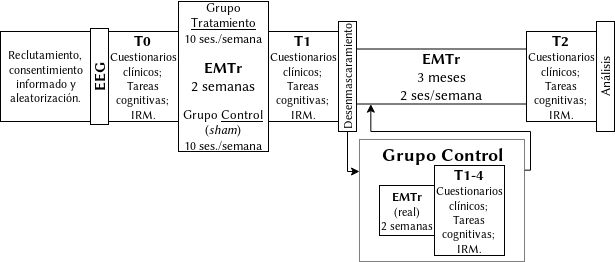
\includegraphics[width=\textwidth]{Des1}
    \caption{Linea de curso del tratamiento clínico de EMTr}
    \label{fig:txTMS}
\end{figure}

\subsubsection{Etapa 0}
Los participantes fueron reclutados dentro y fuera de la clínica de adicciones del INPRFM, buscando a todos aquellos que estuvieran interesados en un tratamiento para la dependencia a la cocaína.
Todos fueron entrevistados por un psiquiatra del instituto sobre los criterios de inclusión y exclusión.
En caso de ser admitidos al estudio, se les explicó completa y detalladamente las características principales del mismo y se les dio a firmar un consentimiento informado.
La asignación a grupos fue realizada por medio de un algoritmo aleatorizado por el director de la unidad y guardado en una memoria USB para cada sujeto que sería introducida directamente al resonador con tal de mantener el estado de doble-ciego.
La evaluación basal (T0) de los pacientes consistió en
\begin{enumerate*}[label=\emph{\alph*}), before=\unskip{: }, itemjoin={{; }}, itemjoin*={{, y }}]
    \item una entrevista clínica semi-estructurada aplicada por un psiquiatra
    \item una batería de escalas clínicas aplicada por un psiquiatra
    \item una batería de tareas cognitivas aplicadas por asistentes de investigación entrenados
    \item una prueba toxicológica de orina
    \item una corrida de MRI.
\end{enumerate*}
A todos los participantes se les aplicó un electroencefalograma para descartar cualquier actividad anómala que pudiera sugerir predisposición a un episodio convulsivo antes de iniciar con la fase de tratamiento.

\subsubsection{Etapa 1}
La primera fase de tratamiento consistió en 20 sesiones de EMTr real o sham a lo largo de 10 días hábiles consecutivos. Cada sesión fue aplicada por un técnico entrenado en la administración de EMTr. Tomó el umbral motor, ubicó la zona de estimulación y se encargo de aplicar los trenes de estimulación y estar al pendiente de posibles efectos adversos.
Los pacientes tuvieron un descanso de 30 minutos entre ambas sesiones.
Al finalizar, el técnico tomó un registro de cualquier molestia y se agendó la cita del siguiente día.\par
Una vez terminadas las 20 sesiones, los pacientes pasaron por otra evaluación (T1) clínica, de orina y MRI, antes de ser revelada su asignación de grupo.

\subsubsection{Etapa 1-4}
A todos aquellos participantes que llevaron estimulación sham se les ofreció continuar con un tratamiento de EMTr por otras 20 sesiones con las mismas características que el grupo de tratamiento real. Una vez concluidas las dos semanas de la fase abierta, una tercera evaluación clínica, de orina y MRI (T1-4) fue realizada.

\subsubsection{Etapa 2}
Esta etapa consistió en la primera fase de sesiones semanales de mantenimiento. Cuando los pacientes terminaron con las 20 sesiones de tratamiento real, se les citó semanalmente para dos sesiones de mantenimiento de EMTr por 10 semanas. Al completar los tres meses de la etapa basal, los pacientes tuvieron otra evaluación clínica, de orina y MRI (T2).

\subsubsection{Etapa 3}
Se continuó el mantenimiento bajo las mismas condiciones por otras 12 semanas hasta completar los seis meses transcurridos desde la etapa basal y llevar a cabo una última evaluación clínica, de orina y MRI (T3).

\section{Instrumentos}
\subsection{Medidas de \textit{craving} y recaída}
\begin{description}
    \item[CCQ-G] Cuestionario de \textit{Craving} de la Cocaína, versión general (\textit{Cocaine Craving Questionnaire, General}); escala que evalúa el deseo intenso hacia la droga de forma promedio en la última semana \parencite{Tiffany1993}.
    \item[CCQ-N] Cuestionario de \textit{Craving} a la Cocaína, versión actual (\textit{Cocaine Craving Questionnaire, Now}); escala que evalúa de forma presente el deseo intenso hacia la droga en el momento de aplicación \parencite{Tiffany1993}.
    \item[VAS] Escala Visual Análoga; escala visual análoga de \SI{100}{\milli\meter} utilizada para representar el \textit{craving} en el momento.
    \item[Línea de tiempo restrospectiva] Calendario de consumo como herramienta para medir el \emph{lapso} (por lo menos un evento de consumo con patrón diferente al basal) y \emph{relapso} (evento de consumo con el mismo patrón que el consumo basal).
\end{description}
\subsection{Medida de impulsividad}
\begin{description}
    \item[BIS-11] Escala de impulsividad de Barratt 11 (Barratt Impulsivity Scale 11); escala clínica que evalúa multidimensionalmente el índice de impulsividad \parencite{H.Patton1995,Salvo2013}.
\end{description}

\section{Estimulación magnética transcraneal repetitiva}
\subsection{Localización de la corteza prefrontal dorsolateral}
El objetivo de la estimulación cortical fue establecido tomando como base puntos de referencia craneales utilizando la distancia teórica entre la región cortical objetivo y un punto en el cuero cabelludo determinado por EMT (procedimiento guiado funcionalmente) \parencite{Sparing2008}.
El área cortical motora izquierda fue el punto de referencia.
M1 fue determinada como la zona en donde hubiera una respuesta motora prominente en el dedo pulgar de la mano contralateral.
El umbral motor (MT) fue definido como la intensidad de estimulación menor que produjera una respuesta motora observable en al menos tres de cinco pulsos.
La localización de la corteza prefrontal dorsolateral fue \SI{5}{\centi\meter} anterior y \SI{2}{\centi\meter} lateral a M1 \parencite{Herwig2001a,Varnava2011a}.

\subsection{Estimulación real}
La EMTr fue aplicada con un estimulador rápido Magpro R-30 MagVenture (Medtronic, Dinamarca) equipado con una bobina MCF-P-B70 en forma de 8 y de \SI{75}{\milli\meter} de diámetro interno en cada espiral, con enfriamiento estático y capacidad de estimulación sham. \par
El centro de la bobina fue colocado sobre la corteza prefrontal dorsolateral izquierda con el asa a \SI{45}{\degree} relativos a la linea media-sagital. \par
La estimulación se aplicó en dos sesiones de EMTr a alta frecuencia (\SI{5}{\hertz}) en un mismo día separadas por un intervalo inter-sesión de \SI{30}{\minute}.
Cada sesión consistió en 50 trenes de \SI{10}{\second} con un intervalo inter-tren de \SI{1}{\minute} a 100\% del umbral motor, dando un total de 5000 pulsos divididos en dos sesiones de \SI{58}{\minute} y de 2500 pulsos.

\subsection{Estimulación sham}
La estimulación sham fue dada con el mismo estimulador y parámetros que la estimulación real. Sin embargo, la bobina fue colocada en su posición sham donde el sonido es idéntico a la estimulación real pero no dispara ningún pulso electromagnético.
A todos los sujetos durante las dos semanas de fase ciega se les colocó un electrodo en el músculo frontal sincronizado con el resonador con el fin de simular la sensación de la estimulación independientemente del grupo de tratamiento y mantener el doble-ciego.

\section{Imagen por resonancia magnética}
\subsection{Adquisición}
Tomamos las imágenes por resonancia magnética con un resonador Philips Ingenia de \SI{3}{\tesla} (Philips, EEUU) y una antena de cráneo de 32 canales. La corrida consistió en una secuencia estructural T1w de alta definición, una secuencia EPI de fMRI en estado de reposo, una secuencia de difusión HARDI-DWI y una secuencia experimental FAST-DKI. Para la presente investigación, solo utilizamos las secuencias funcional y la estructural.\par
Para la secuencia funcional, a los pacientes se les instruyó que se recostaran en el resonador moviéndose lo menos posible, que no pensaran en nada en específico y mantuvieran los ojos abiertos. Una cruz de fijación fue proyectada durante los \SI{10}{/minute} de secuencia funcional, pero se les explicó que no tenían que enfocarse en esta. \par
La fMRI fue tomada con una secuencia EPI (eco-planar) T2* con los siguientes parámetros
\begin{enumerate*}[label=\emph{\alph*}), before=\unskip{: }, itemjoin={{; }}, itemjoin*={{, y }}]
    \item TR = \SI{2}{\second}
    \item TE = \SI{30}{\milli\second}
    \item ángulo de inclinación de \SI{75}{\degree}
    \item 37 cortes de \SI{3.33}{\milli\meter} de grosor sin espacio entre corte
    \item FOV = \SI{240}{\milli\meter}
    \item matriz de \num{80x80}
    \item voxel de \SI[product-units=single]{3x3x3.33}{\milli\meter}.
\end{enumerate*}
Una secuencia \textit{fieldmap} fue tomada en dirección opuesta para el preprocesamiento.\par
La secuencia 3D de alta resolución T1w fue adquirida con los siguientes parámetros
\begin{enumerate*}[label=\emph{\alph*}), before=\unskip{: }, itemjoin={{; }}, itemjoin*={{, y }}]
    \item TR = \SI{7}{\milli\second}
    \item TE = \SI{3.5}{\milli\second}
    \item ángulo de inclinación de \SI{8}{\degree}
    \item 180 cortes de \SI{1}{\milli\meter} de grosor sin espacio entre corte
    \item FOV = \SI{240}{\milli\meter}
    \item matriz de \num{240x240}
    \item voxel de \SI[product-units=single]{1}{\milli\meter\cubed}.
\end{enumerate*}

\subsection{Manejo de datos}
Los datos de imagen fueron extraídos del formato \texttt{DICOM}, transformados a \texttt{NIfTI} y organizados en \texttt{BIDS} \parencite{Gorgolewski2016}.
La calidad de los datos fue evaluada con \texttt{MRIQC} \parencite{Esteban2017} para evaluar posibles artefactos de señal y/o movimiento. Los datos de neuroimagen de los controles sanos retomados de la investigación de \parencite{Garza2017} siguieron la misma línea de trabajo descrita a continuación.\par

\subsection{Preprocesamiento de datos}
Las imágenes fueron preprocesadas utilizando \texttt{FMRIPREP v1.4.1} \parencite{Esteban2019}, una herramienta basada en \texttt{Nipype} \parencite{Gorgolewski2011}.
Cada volumen de las imágenes T1w fue corregido por INU (no-uniformidad en intensidad) usando \texttt{N4BiasFieldCorrection v2.1.0} \parencite{Tustison2010} y se les removió el cráneo con \texttt{antsBrainExtraction.sh v2.1.0} (con la plantilla OASIS).
La normalización espacial a la plantilla ICBM 152 asimétrica no-lineal versión 2009c \parencite{Fonov2009} fue realizada por medio de un registro no-lineal con \texttt{antsRegistration} de \texttt{ANTs v2.1.0} \parencite{Avants2008}, usando versiones sin cráneo tanto del volumen T1w como de la plantilla.
La segmentación del tejido cerebral del líquido cefalorraquídeo (LCR), sustancia blanca (WM) y gris (GM) fue realizada en la imagen T1w sin cráneo usando \texttt{fast} de \texttt{FSL v.5.0.9} \parencite{Zhang2001}.\par
Los datos funcionales fueron corregidos por el tiempo de corte usando \texttt{3dTshift} de \texttt{AFNI v16.2.07} \parencite{Cox1996} y por movimiento con \texttt{mcflirt} (\texttt{FSL v5.0.9} \parencite{Jenkinson2002}.
Esto fue seguido por un corregistro al volumen T1w correspondiente usando un registro basado-en-límites \parencite{Greve2009} con seis grados de libertad, usando \texttt{bbregister} (\texttt{FreeSurfer v6.0.1}).
Las transformaciones para corregir movimiento, transformación BOLD-a-T1w y deformación T1w-a-plantilla (MNI) fueron concatenadas y aplicadas en un solo paso usando \texttt{antsApplyTransforms} \texttt{(ANTS v2.1.0)} usando interpolación Lanczos.\par
Una máscara para excluir señal con origen cortical fue obtenida erosionando la máscara del cerebro, asegurándose de que solo se contuvieran estructuras subcorticales.
Seis componentes tCompCor fueron entonces calculados incluyendo solo el top 5\% de voxeles variables dentro de la máscara subcortical.
Para aCompCor, seis componentes fueron calculados en el espacio T1w, después de su proyección al espacio nativo de cada corrida funcional.
El desplazamiento de marco (FD, \textit{frame-wise displacemente}) \parencite{Power2014} fue calculado para cada corrida funcional usando la implementación de \texttt{Nipype}.\par
Muchas operaciones internas de \texttt{FMRIPREP} usan \texttt{Nilearn} \parencite{Abraham2014}, principalmente dentro del flujo de trabajo del procesamiento BOLD. Para más detalles del trabajo de preprocesamiento ver \url{https://fmriprep.readthedocs.io/en/latest/workflows.html}.\par
Una vez obtenidas las matrices de regresiones de ruido de \texttt{FMRIPREP} los datos fueron preprocesados con la herramienta \texttt{xcpEngine} \parencite{Ciric2017}.
Debido a la naturaleza clínica de la muestra y las altas tasas de movimiento (medido por FD), utilizamos la estrategia de preprocesamiento de \textcite{Power2014} de 36 parámetros de regresión y \textit{scrubbing} (eliminación de los volúmenes que sobrepasen un umbral de FD establecido; en nuestro caso de \SI{0.5}{\milli\meter}).

\subsection{Construcción de redes}
Por medio de la misma herramienta de procesamiento \texttt{xcpEngine} se extrajeron las lineas de tiempo de la señal BOLD de cada uno de los 264 nodos del atlas funcional de \parencite{Power2011} basado en un meta-análisis de datos de fMRI de tareas.\par
Utilizando \texttt{R v3.5.3} \parencite{R2019,Rstudio2018} creamos matrices de  adyacencia obteniendo el coeficiente de correlación de Pearson $r$ de la señal BOLD entre cada una de las áreas de la parcelación.\par
Posteriormente con la intención de eliminar conexiones espúreas y disminuir el ruido dentro de las redes, aplicamos un método de umbralización de consenso donde se reconstruyen las matrices de adyacencia incluyendo solo las conexiones cuyo peso de conexión, o \emph{fuerza}, igualara o excediera un umbral grupal establecido:
\begin{equation}
    \label{eqn:threshold}
    w_{ij}=
    \begin{cases}
        w_{ij}, & \text{si}\ w_{ij} \geq \tau \enspace \text{en}\ (\frac{T}{100})m \\
        0, & \text{de otra forma}
    \end{cases}
\end{equation}
dado un umbral grupal $T$ (expresado como porcentaje) y una muestra de redes cerebrales $m$, una arista es tomada como presente en la reconstrucción de la matriz si sobrepasa un umbral de conectividad $\tau$ en al menos $\frac{T}{100}m$ \parencite{DeReus2013}. \par
Para esta investigación los parámetros utilizados fueron $\tau = 0.25$ y $T = 50\%$; es decir, toda arista debía tener un valor de correlación igual o mayor a $0.25r$ en al menos la mitad de los integrantes del grupo para permanecer en la matriz reconstruida.\par
Del mismo modo, todas las auto-conexiones y conexiones negativas (anti-correlaciones funcionales) fueron retiradas de las matrices antes del análisis \parencite{Rubinov2010}.

\subsection{Medidas topológicas}
Teniendo las matrices de adyacencia finales, los grafos de la red de conectividad funcional para cada sujeto fueron creados con la paquetería \texttt{brainGraph v2.2} \parencite{Watson2018}. Para cada grafo se extrajeron las siguientes medidas topológicas
\begin{enumerate*}[label=\emph{\alph*}), before=\unskip{: }, itemjoin={{; }}, itemjoin*={{, y }}]
    \item grado
    \item densidad
    \item coeficiente de agrupamiento
    \item longitud de camino característica
    \item eficiencia local
    \item eficiencia global
    \item escalar de mundo pequeño
\end{enumerate*}.

\subsection{Redes aleatorias}
Una vez construidos los grafos a partir de las matrices de adyacencia umbralizadas, con el fin de calcular las medidas de mundo pequeño, se crearon 300 redes con el mismo número de nodos y grado de conectividad siguiendo el procedimiento propuesto por \textcite{Maslov2002}. De estas redes se obtuvieron las medidas $L^w_g$ y $C^w_g$ para posteriormente calcular $\lambda_g$ (formula \ref{eqLambda}), $\gamma_g$ (formula \ref{eqGamma}) y el escalar de mundo pequeño $\sigma$ (formula \ref{eqSW}).

\section{Análisis de datos}
Todos los análisis estadísticos fueron hechos dentro del entorno de programación para \texttt{R} \texttt{RStudio} \parencite{Rstudio2018}.

Para el presente proyecto se realizaron cuatro análisis distintos.

\subsection{Análisis 1: Exploración transversal de controles}
Debido a la escasa investigación sobre la naturaleza de la topología de redes de conectividad funcional en sujetos con dependencia a la cocaína, se realizó una comparación transversal de las diferencias en las métricas de topología de red entre los 46 pacientes diagnosticados con dependencia a la cocaína que tuvieron una medición basal y los datos retomados de los 45 controles sanos.
En un análisis exploratorio observamos las distintas métricas de topología de red a lo largo de los distintos valores de $\tau$ de umbralizaje. Posteriormente se realizaron distintas regresiones lineales multivariadas para cada métrica de interés (fuerza, densidad, eficiencia local, eficiencia global y métrica de mundo pequeño). Las variables demográficas de edad, sexo y nivel educativo fueron incluidos como covariantes.

\subsection{Análisis 2: Fase cerrada}
Dado a la asignación grupal aleatoria del estudio, optamos por no explorar las diferencias demográficas y atribuirlas a efectos aleatorios.
Exploramos la relación entre los puntajes reportados en las distintas escalas clínicas por medio de una correlación de pearson.
Ambos grupos (estimulación real y estimulación sham) fueron subdivididos a su vez por medio de la mediana del puntaje basal reportado por cada escala y por grupo con la intención de diferenciar los patrones de cambio de los pacientes que comenzaron el tratamiento con una sintomatología elevada de quienes mostraron una sintomatología leve.
La eficacia del tratamiento fue explorada utilizando regresiones lineales multivariadas para cada escala (VAS, CCQ-G, CCQ-N y BIS-11) usando el grupo de estimulación como predictor y las medidas clínicas basales como covariantes.
Los cambios en topología de red fueron analizados por medio de modelos de efectos mixtos. Para cada métrica de red, se realizó un modelo distinto buscando la interacción de fase de tratamiento y grupo de estimulación. Además se introdujeron las medidas clínicas y las variables demográficas de edad, sexo y nivel educativo como covariantes.

\subsection{Análisis 3: Fase abierta (3 meses)}
De forma exploratoria se analizaron los cambios observados posteriores a 3 meses de sesiones semanales de mantenimiento en aquellos sujetos que llegaron hasta la fase T2.
Tanto las escalas clínicas como las métricas de red fueron exploradas por medio de modelos de efectos mixtos buscando la diferencia entre las distintas fases de la medición basal e incluyendo las variables demográficas de edad, sexo y nivel educativo como covariantes; para los modelos de las métricas topológicas además se incluyeron los puntajes clínicos.

\subsection{Análisis 4: Fase abierta (6 meses)}
Para obtener una medición más objetiva, se decidió separar el análisis longitudinal de mantenimiento en las mediciones a tres y seis meses. Para este segundo análisis, nos enfocamos únicamente en aquellos participantes que completaron todas las fases del estudio y exploramos sus cambios a lo largo de estas.
De igual forma que el análisis a 3 meses, por medio de modelos de efectos mixtos se exploraron las diferencias con respecto a la medición basal incluyendo edad, sexo y nivel educativo como covariantes.



\backmatter
\addcontentsline{toc}{chapter}{\bibname}
\printbibliography
\end{document}

